\documentclass[a4paper]{article}
\setlength{\parindent}{0pt}

%%%%%%%% CREATE DOCUMENT STRUCTURE %%%%%%%%
%% Language and font encodings
\usepackage[english]{babel}
\usepackage[utf8x]{inputenc}
\usepackage[T1]{fontenc}
%\usepackage{subfig}

%% Sets page size and margins
\usepackage[a4paper,top=3cm,bottom=2cm,left=2cm,right=2cm,marginparwidth=1.75cm]{geometry}

%% Useful packages
\usepackage{framed}
\usepackage{amsmath}
\usepackage{graphicx}
%\usepackage[colorinlistoftodos]{todonotes}
\usepackage[colorlinks=true, allcolors=blue]{hyperref}
\usepackage{caption}
\usepackage{subcaption}
\usepackage{listings}
\usepackage{lstautogobble}
\usepackage{sectsty}
\usepackage{apacite}
\usepackage{float}
\usepackage{titling} 
\usepackage{blindtext}
\usepackage[square,sort,comma,numbers]{natbib}
\usepackage{xcolor}
\definecolor{darkgreen}{rgb}{0.0, 0.4, 0.0}

\definecolor{pblue}{rgb}{0.13,0.13,1}
\definecolor{pgreen}{rgb}{0,0.5,0}
\definecolor{pred}{rgb}{0.9,0,0}
\definecolor{pgrey}{rgb}{0.46,0.45,0.48}

\usepackage{listings}
\lstset{language=Java,
    showspaces=false,
    showtabs=false,
    breaklines=true,
    showstringspaces=false,
    breakatwhitespace=true,
    commentstyle=\color{pgreen},
    keywordstyle=\color{pblue},
    stringstyle=\color{pred},
    basicstyle=\ttfamily,
    colframe=white!75!black,
    moredelim=[is][\textcolor{pgrey}]{\%\%}{\%\%}
}

\usepackage[most]{tcolorbox}

\newtcblisting{shell}{colback=black,colupper=white,colframe=white!75!black,
	listing only,listing options={language=sh}}

% ToDo: List
\usepackage{enumitem,amssymb}
\newlist{todolist}{itemize}{2}
\setlist[todolist]{label=$\square$}

\usepackage{tikz}
\usetikzlibrary{calc,shapes.multipart,chains,arrows}

%%%%%%%% DOCUMENT %%%%%%%%
\begin{document}

%%%% Title Page
\begin{titlepage}

\newcommand{\HRule}{\rule{\linewidth}{0.5mm}} 							% horizontal line and its thickness
\center 
 
 
% University
\textsc{\LARGE University of Illinois @ Urbana-Champaign}\\[1cm]

% Document info
\textsc{\Large CI 487: Data Structures for CS Teachers}\\[0.2cm]
\textsc{\large }\\[1cm] 										% Course Code
\HRule \\[0.8cm]
{ \huge \bfseries Implementation \#3:\\\vspace{0.1cm}Implementing a Generic Singly Linked List}\\[0.7cm]								% Assignment
\HRule \\[0.8cm]
%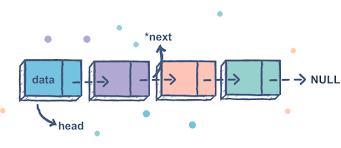
\includegraphics[width=0.6\textwidth]{images/singly-linked-list.png}\\[1cm] 	% University logo
\vfill 
\end{titlepage}

%%\begin{abstract}
%%Your abstract.
%%\end{abstract}

%%%% SECTIONS
%% Section 1
\section{Objectives and Overview}

This assignment covers the following
\begin{itemize}
    \item Nested vs Inner classes
    \item Singly linked-list structure and operations
    \item Another implementation of generic data-structures
\end{itemize}

\textbf{NOTE:} Complete all methods in the order they are presented. Do NOT
move onto impelementing another method before completing one and testing it.
With previous assignment you might have been able to get away with jumping between
implementing different methods however as we move into the world of lists and trees
doing this without testing and debugging can lead to compounding errors which are 
difficulty to debug.

\section{Structures and Specifications}

For this assignment you will only be implementing one \lstinline|.java| file in
addition to \lstinline|main|. The \lstinline|SinglyLinkedList<E>| class will be
the class that represents our linked list as a whole and allows for operations
to be performed on that linked list. The individual elements of our linked-list
will be represented by the \lstinline|ListNode<E>| class which will be a
\textit{static inner} class of \lstinline|SinglyLinkedList<E>|.

\subsection{Nested vs Inner Classes (\href{https://docs.oracle.com/javase/tutorial/java/javaOO/nested.html}{docs})}
\begin{minipage}{0.45\textwidth}
\begin{lstlisting}[frame=trBL]
class OuterClass{
    class InnerClass{
        //...
    }
}
\end{lstlisting}
\end{minipage}
\hfill
\begin{minipage}{0.45\textwidth}
\begin{lstlisting}[frame=trBL]
class OuterClass{
    static class NestedClass{
        //...
    }
}
\end{lstlisting}
\end{minipage}

In Java there are two ways of embedding classes within other classes:
\begin{itemize}
    \item \textbf{Inner Class:} This is a class that been declared within another class without the \lstinline|static| modifier. It has access to all of the methods and attributes \textit{regardless of the access modifier they were declared with.} That is to say, the inner class has access to all of the outer classes private variables and methods. Additionaly, you must first instantiate the outer class before instantiating the inner class.
    \item \textbf{Nested Class:} A nested class is similar to an inner class but is instead declared \textit{with} a \lstinline|static| modifier. This separates them more from their outer class and does not allow the nested class access to it's outer classes \lstinline|private| variables. Declaring the embedded class as \lstinline|static| also allows it to be instantiated regardless of whether its outer class has been instantiated. 
\end{itemize}
In both cases these classes are declared for packaging convinience and the
embedded classes are small classes that are only of utility to their outer
class. Our \lstinline|ListNode<E>| class is an example of this since it has no
real utility outside the contex of it's usage in \lstinline|SinglyLinkedList<E>|. It 
also doesn't need to access any of it's outer classes variables or methods 
so it makes sense to declare it as a \textit{nested class} rather than an
\textit{inner class}. This leaves us with the following class structure
for our linked-list.\\

\begin{lstlisting}[frame=trBL]
class SinglyLinkedList<E>{
    static class ListNode<E>{
        //...
    }
}
\end{lstlisting}


\newpage


\section{Step 0: Understanding what you are given}

Before you begin it is important to understand the code you have been given and it's functionality. 
As such, \textit{your are highly encouraged} to read through the existing code in the SinglyLinkedListText.java
file as well as the provided code in SinglyLinkedList.java, the latter of which is described below.

\subsection{ListNode}

\begin{figure}[H]
    \centering
    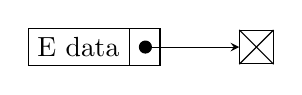
\begin{tikzpicture}[list/.style={rectangle split, rectangle split parts=2, draw, rectangle split horizontal}, >=stealth, start chain]

        \node[list,on chain] (A) {E data};

        \node[on chain,draw,inner sep=6pt] (N) {};
        \draw (N.north east) -- (N.south west);
        \draw (N.north west) -- (N.south east);

        \draw[*->] let \p1 = (A.two), \p2 = (A.center) in (\x1,\y2) -- (N);

    \end{tikzpicture}
    \caption{Example ListNode}
    \label{fig:listnode}
\end{figure}


\subsubsection{Attributes}

\begin{enumerate}
    \item \lstinline|E data|: A reference to a generic data. Leave it at the default access level.
    \item \lstinline|ListNode<E> next|: A reference to the next node in the list. Leave it at the default access level.
\end{enumerate}

And that's it! This class doesn't have any methods just for simplicity's sake
since it's only purpose is to store the data associated with elements of the
linked-list.  An example of how list nodes will be represented in future
diagrams can be seen in Figure~\ref{fig:listnode}. This node has some generic
\lstinline|data| and the \lstinline|next| attribute is initially
\lstinline|null| (depicted as pointing to a box with an X). 

\subsubsection{Constructor}

The constructor for this class takes a single, generic parameter.  It
initializes the \lstinline|data| attribute with the parameter and initializes
the \lstinline|next| node to be null.

\subsection{SinglyLinkedList}

\begin{figure}[H]
    \centering
    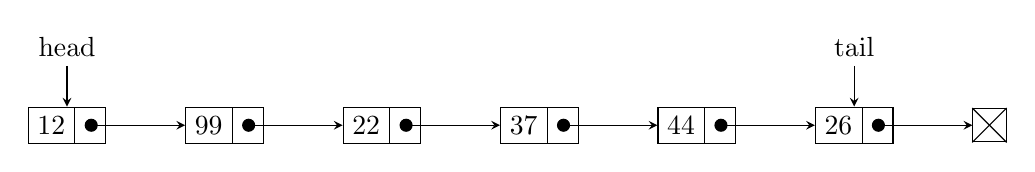
\begin{tikzpicture}[list/.style={rectangle split, rectangle split parts=2, draw, rectangle split horizontal}, >=stealth, start chain]

        \node[list,on chain] (A) {12};
        \node[list,on chain] (B) {99};
        \node[list,on chain] (C) {22};
        \node[list,on chain] (D) {37};
        \node[list,on chain] (E) {44};
        \node[list,on chain] (F) {26};


        \node[above of=A] (H) {head};
        \node[above of=F] (T) {tail};

        \node[on chain,draw,inner sep=6pt] (N) {};
        \draw (N.north east) -- (N.south west);
        \draw (N.north west) -- (N.south east);


        \draw[*->] let \p1 = (A.two), \p2 = (A.center) in (\x1,\y2) -- (B);
        \draw[*->] let \p1 = (B.two), \p2 = (B.center) in (\x1,\y2) -- (C);
        \draw[*->] let \p1 = (C.two), \p2 = (C.center) in (\x1,\y2) -- (D);
        \draw[*->] let \p1 = (D.two), \p2 = (D.center) in (\x1,\y2) -- (E);
        \draw[*->] let \p1 = (E.two), \p2 = (E.center) in (\x1,\y2) -- (F);
        \draw[*->] let \p1 = (F.two), \p2 = (F.center) in (\x1,\y2) -- (N);

        \draw[->] (H) -- (A);
        \draw[->] (T) -- (F);


    \end{tikzpicture}\\
    \caption{A visual represention of this class as a chain of \lstinline|ListNode<E>| instances along with a \lstinline|head| and \lstinline|tail| reference.}
    \label{fig:singlylinkedlist}
\end{figure}


\subsubsection{Attributes}

\begin{enumerate}
    \item \lstinline|ListNode<E> head|: This is a reference to the first node in the linked list. This has a \lstinline|private| access level as we don't want users of the class to directly modify it. Rather, we want to control their access via the add/remove methods.
    \item \lstinline|ListNode<E> tail|: A reference to the last node in the linked list. This should have a \lstinline|private| access level for the same reasons as stated above
    \item \lstinline|int size|: The current number of nodes in the list. This should have a \lstinline|private| access level as the class provides a \lstinline|size()| method with allows read access but no setter so the user of the class can't directly modify it.
\end{enumerate}

\subsubsection{Constructor}

Your linked-list class has the following constructor:
\begin{enumerate}
    \item \lstinline|public SinglyLinkedList(E data)|: This constructor initializes \lstinline|head| and \lstinline|tail| attributes to \lstinline|null| and set the initial size of the linked-list to 0. This is because, upon initially creating the list it is empty.
\end{enumerate}


\newpage
\section{Step 1: Implementing the addToFront and addToEnd Methods}


\begin{figure}[H]
    \begin{minipage}{0.48\textwidth}
    \centering
    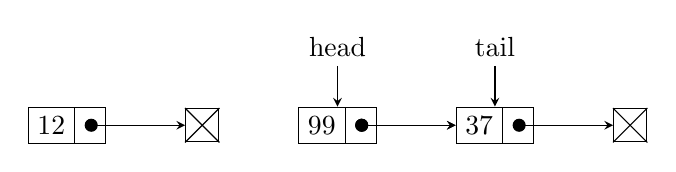
\begin{tikzpicture}[list/.style={rectangle split, rectangle split parts=2, draw, rectangle split horizontal}, >=stealth, start chain]

        \node[list,on chain] (A) {12};

        \node[on chain,draw,inner sep=6pt] (N1) {};
        \draw (N1.north east) -- (N1.south west);
        \draw (N1.north west) -- (N1.south east);

        \node[list,on chain] (B) {99};
        \node[list,on chain] (C) {37};
        \node[above of=B] (H) {head};
        \node[above of=C] (T) {tail};
        \node[on chain,draw,inner sep=6pt] (D) {};
        \draw (D.north east) -- (D.south west);
        \draw (D.north west) -- (D.south east);
        \draw[*->] let \p1 = (A.two), \p2 = (A.center) in (\x1,\y2) -- (N1);
        \draw[*->] let \p1 = (B.two), \p2 = (B.center) in (\x1,\y2) -- (C);
        \draw[*->] let \p1 = (B.two), \p2 = (B.center) in (\x1,\y2) -- (C);
        \draw[*->] let \p1 = (C.two), \p2 = (C.center) in (\x1,\y2) -- (D);
        \draw[->] (H) -- (B);
        \draw[->] (T) -- (C);

    \end{tikzpicture}\\
    \textbf{Step 1: Instantiate a new ListNode}
\end{minipage}
\hfill
\begin{minipage}{0.48\textwidth}
    \centering
    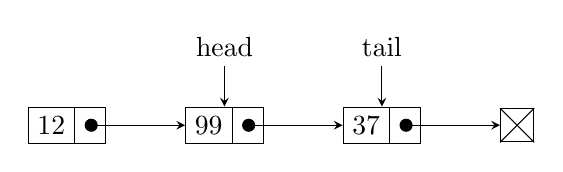
\begin{tikzpicture}[list/.style={rectangle split, rectangle split parts=2, draw, rectangle split horizontal}, >=stealth, start chain]

        \node[list,on chain] (A) {12};
        \node[list,on chain] (B) {99};
        \node[list,on chain] (C) {37};
        \node[above of=B] (H) {head};
        \node[above of=C] (T) {tail};
        \node[on chain,draw,inner sep=6pt] (D) {};
        \draw (D.north east) -- (D.south west);
        \draw (D.north west) -- (D.south east);
        \draw[*->] let \p1 = (A.two), \p2 = (A.center) in (\x1,\y2) -- (B);
        \draw[*->] let \p1 = (B.two), \p2 = (B.center) in (\x1,\y2) -- (C);
        \draw[*->] let \p1 = (C.two), \p2 = (C.center) in (\x1,\y2) -- (D);
        \draw[->] (H) -- (B);
        \draw[->] (T) -- (C);

    \end{tikzpicture}\\
    \textbf{Step 2: Add the node to the front of the list}
\end{minipage}\\
\vspace{0.25cm}\\
\begin{minipage}{\textwidth}
    \centering
    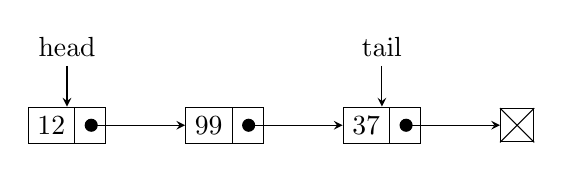
\begin{tikzpicture}[list/.style={rectangle split, rectangle split parts=2, draw, rectangle split horizontal}, >=stealth, start chain]

        \node[list,on chain] (A) {12};
        \node[list,on chain] (B) {99};
        \node[list,on chain] (C) {37};
        \node[above of=A] (H) {head};
        \node[above of=C] (T) {tail};
        \node[on chain,draw,inner sep=6pt] (D) {};
        \draw (D.north east) -- (D.south west);
        \draw (D.north west) -- (D.south east);
        \draw[*->] let \p1 = (A.two), \p2 = (A.center) in (\x1,\y2) -- (B);
        \draw[*->] let \p1 = (B.two), \p2 = (B.center) in (\x1,\y2) -- (C);
        \draw[*->] let \p1 = (C.two), \p2 = (C.center) in (\x1,\y2) -- (D);
        \draw[->] (H) -- (A);
        \draw[->] (T) -- (C);

    \end{tikzpicture}\\
    \textbf{Step 3: Update the head reference to be the new front of the list}
\end{minipage}


    \caption{Adding a node to the front of a non-empty LinkedList}
    \label{fig:addtofront}
\end{figure}

\paragraph{\lstinline|public void addToFront(E data)|: } This method takes a
single generic parameter, generates a new \lstinline|ListNode<E>| with that
data, and adds it to the front of the linked list. When making this method you
should consider two sub-cases: (1) the linked-list is empty and (2) the linked
list contains nodes. In the case the linked list is empty (i.e.,
\lstinline|head| == \lstinline|null|) you will want to set the tail and the head
equal to the new node. Otherwise, you will want to set the new node's next reference 
equal to the current \lstinline|head|, update the \lstinline|head| to be the new node,
and increment the size attribute to indicate a new node has been added (see
Figure~\ref{fig:addtofront}).\\

\begin{figure}[H]
\begin{minipage}{0.48\textwidth}
    \centering
    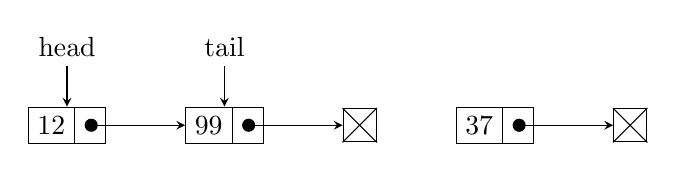
\begin{tikzpicture}[list/.style={rectangle split, rectangle split parts=2, draw, rectangle split horizontal}, >=stealth, start chain]

        \node[list,on chain] (A) {12};

        \node[list,on chain] (B) {99};

        \node[on chain,draw,inner sep=6pt] (N1) {};
        \draw (N1.north east) -- (N1.south west);
        \draw (N1.north west) -- (N1.south east);

        \node[list,on chain] (C) {37};

        \node[above of=A] (H) {head};
        \node[above of=B] (T) {tail};

        \node[on chain,draw,inner sep=6pt] (D) {};
        \draw (D.north east) -- (D.south west);
        \draw (D.north west) -- (D.south east);
        \draw[*->] let \p1 = (A.two), \p2 = (A.center) in (\x1,\y2) -- (B);
        \draw[*->] let \p1 = (B.two), \p2 = (B.center) in (\x1,\y2) -- (N1);
        \draw[*->] let \p1 = (C.two), \p2 = (C.center) in (\x1,\y2) -- (D);

        \draw[->] (H) -- (A);
        \draw[->] (T) -- (B);

    \end{tikzpicture}\\
    \textbf{Step 1: Instantiate a new ListNode}
\end{minipage}
\hfill
\begin{minipage}{0.48\textwidth}
    \centering
    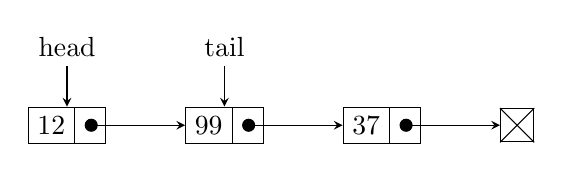
\begin{tikzpicture}[list/.style={rectangle split, rectangle split parts=2, draw, rectangle split horizontal}, >=stealth, start chain]

        \node[list,on chain] (A) {12};

        \node[list,on chain] (B) {99};

        \node[list,on chain] (C) {37};

        \node[above of=A] (H) {head};
        \node[above of=B] (T) {tail};

        \node[on chain,draw,inner sep=6pt] (D) {};
        \draw (D.north east) -- (D.south west);
        \draw (D.north west) -- (D.south east);
        \draw[*->] let \p1 = (A.two), \p2 = (A.center) in (\x1,\y2) -- (B);
        \draw[*->] let \p1 = (B.two), \p2 = (B.center) in (\x1,\y2) -- (C);
        \draw[*->] let \p1 = (C.two), \p2 = (C.center) in (\x1,\y2) -- (D);

        \draw[->] (H) -- (A);
        \draw[->] (T) -- (B);

    \end{tikzpicture}\\
    \textbf{Step 2: Add the node to the end of the list}
\end{minipage}\\
\vspace{0.25cm}\\
\begin{minipage}{\textwidth}
    \centering
    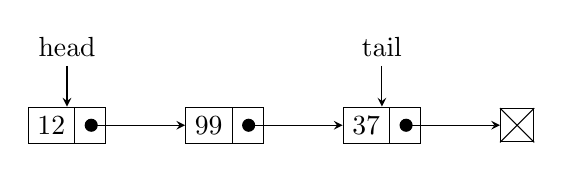
\begin{tikzpicture}[list/.style={rectangle split, rectangle split parts=2, draw, rectangle split horizontal}, >=stealth, start chain]

        \node[list,on chain] (A) {12};

        \node[list,on chain] (B) {99};

        \node[list,on chain] (C) {37};

        \node[above of=A] (H) {head};
        \node[above of=C] (T) {tail};

        \node[on chain,draw,inner sep=6pt] (D) {};
        \draw (D.north east) -- (D.south west);
        \draw (D.north west) -- (D.south east);
        \draw[*->] let \p1 = (A.two), \p2 = (A.center) in (\x1,\y2) -- (B);
        \draw[*->] let \p1 = (B.two), \p2 = (B.center) in (\x1,\y2) -- (C);
        \draw[*->] let \p1 = (C.two), \p2 = (C.center) in (\x1,\y2) -- (D);

        \draw[->] (H) -- (A);
        \draw[->] (T) -- (C);

    \end{tikzpicture}\\
    \textbf{Step 3: Update the tail reference to be the front of the list}
\end{minipage}



\caption{Adding a node to the end of a non-empty LinkedList}
\label{fig:addtoback}
\end{figure}


\paragraph{\lstinline|public void addToEnd(E data)|: } For this method you will
be adding to the end of the end of the list. This operation should be fairly
similar to the \lstinline|addToFront| method in that you should consider the
following two cases: (1) the linked-list is empty and (2) the linked-list
contains some nodes. You will begin by instantiating a new node using the 
data passed in as a parameter. Next, if the \lstinline|head| is \lstinline|null|,
we want to set both the \lstinline|head| and the \lstinline|tail| to equal 
the newly created node. If the list is non empty, we want to set the new node
be the current \lstinline|tail|'s next node and then update \lstinline|tail| to 
be the new node since it is now at the end of the list (see Figure~\ref{fig:addtoback}).

\subsection*{Testing}
You have provided test cases for both of the above methods. Upon running the
\texttt{SinglyLInkedListTest.java} file
\begin{shell}
addToFront tests
List 1: 3 --> 2 --> 1 --> null
------------------------------------------

addToEnd tests
List 2: 1 --> 2 --> 3 --> null
------------------------------------------
\end{shell}

\newpage

\section{Step 2: getNodeAtPosition}

Much like the \lstinline|indexOf| method in the last assignment you will find
the following method quite useful, particularly when getting nodes that occur
before other nodes. For example, if we want to add a node at a given
\lstinline|pos| we need a reference to the node that precedes it. This can be
done by calling the method below as: \lstinline|getNodeAtPosition(pos -1)|.
This is why we are implementing this method now given it will greatly simplify
our code later on.

\paragraph{\lstinline|public ListNode<E> getNodeAtPosition(int pos)|} This
method should return a reference to a node at a given position (\lstinline|pos|). In the event
the position (\lstinline|pos|) exceeds the last valid index or the position is
negative of the list this method should throw an
\lstinline|IndexOutOfBoundsException|. Otherwise, you should create a
\lstinline|tmp| pointer to the head, advance it \lstinline|pos| number of
times, and return \lstinline|tmp|.\\

\subsection*{Testing}
The provided tests for get node at position should output the following after you have implemented this method:
\begin{shell}
getNodeAtPosition Tests
The node containing 1 is at position 0 in List 2
The node containing 2 is at position 1 in List 2
The node containing 3 is at position 2 in List 2
------------------------------------------
\end{shell}
As was the case with the last one, you should review the test code in
SinglyLinkedListTest.java and add a few more.

\newpage

\section{Step 3: addNodeAtPosition}

\begin{figure}[H]
\begin{minipage}{\textwidth}
    \centering
    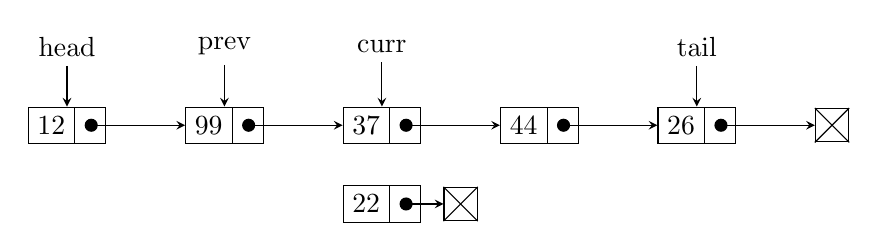
\begin{tikzpicture}[list/.style={rectangle split, rectangle split parts=2, draw, rectangle split horizontal}, >=stealth, start chain]

        \node[list,on chain] (A) {12};
        \node[list,on chain] (B) {99};
        \node[list,on chain] (C) {37};
        \node[list,on chain] (D) {44};
        \node[list,on chain] (E) {26};

        \node[list, below of=C] (New) {22};
        \node[draw,inner sep=6pt, right of=New] (N1) {};
        \draw (N1.north east) -- (N1.south west);
        \draw (N1.north west) -- (N1.south east);
        \draw[*->] let \p1 = (New.two), \p2 = (New.center) in (\x1,\y2) -- (N1);

        \node[above of=A] (H) {head};
        \node[above of=E] (T) {tail};

        \node[above of=C] (Curr) {curr};
        \node[above of=B] (Prev) {prev};

        \node[on chain,draw,inner sep=6pt] (N) {};
        \draw (N.north east) -- (N.south west);
        \draw (N.north west) -- (N.south east);

        \draw[*->] let \p1 = (A.two), \p2 = (A.center) in (\x1,\y2) -- (B);
        \draw[*->] let \p1 = (B.two), \p2 = (B.center) in (\x1,\y2) -- (C);
        \draw[*->] let \p1 = (C.two), \p2 = (C.center) in (\x1,\y2) -- (D);
        \draw[*->] let \p1 = (D.two), \p2 = (D.center) in (\x1,\y2) -- (E);
        \draw[*->] let \p1 = (E.two), \p2 = (E.center) in (\x1,\y2) -- (N);

        \draw[->] (Curr) -- (C);
        \draw[->] (Prev) -- (B);

        \draw[->] (H) -- (A);
        \draw[->] (T) -- (E);

    \end{tikzpicture}\\
    \textbf{Step 1: Search for and find a reference to the node you want to remove and the node that precedes it.}
\end{minipage}
\begin{minipage}{\textwidth}
    \centering
    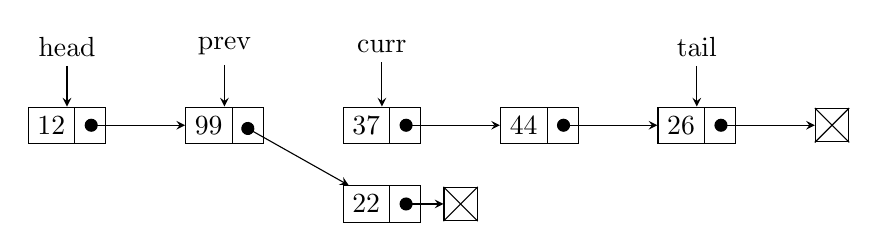
\begin{tikzpicture}[list/.style={rectangle split, rectangle split parts=2, draw, rectangle split horizontal}, >=stealth, start chain]

        \node[list,on chain] (A) {12};
        \node[list,on chain] (B) {99};
        \node[list,on chain] (C) {37};
        \node[list,on chain] (D) {44};
        \node[list,on chain] (E) {26};

        \node[list, below of=C] (New) {22};
        \node[draw,inner sep=6pt, right of=New] (N1) {};
        \draw (N1.north east) -- (N1.south west);
        \draw (N1.north west) -- (N1.south east);
        \draw[*->] let \p1 = (New.two), \p2 = (New.center) in (\x1,\y2) -- (N1);

        \node[above of=A] (H) {head};
        \node[above of=E] (T) {tail};

        \node[above of=C] (Curr) {curr};
        \node[above of=B] (Prev) {prev};

        \node[on chain,draw,inner sep=6pt] (N) {};
        \draw (N.north east) -- (N.south west);
        \draw (N.north west) -- (N.south east);

        \draw[*->] let \p1 = (A.two), \p2 = (A.center) in (\x1,\y2) -- (B);
        \draw[*->] let \p1 = (B.two), \p2 = (B.center) in (\x1,\y2) -- (New);
        \draw[*->] let \p1 = (C.two), \p2 = (C.center) in (\x1,\y2) -- (D);
        \draw[*->] let \p1 = (D.two), \p2 = (D.center) in (\x1,\y2) -- (E);
        \draw[*->] let \p1 = (E.two), \p2 = (E.center) in (\x1,\y2) -- (N);

        \draw[->] (Curr) -- (C);
        \draw[->] (Prev) -- (B);

        \draw[->] (H) -- (A);
        \draw[->] (T) -- (E);

    \end{tikzpicture}\\
    \textbf{Step 2: Update previous node's next node to be a reference to the new node.}
\end{minipage}\\
\vspace{0.25cm}\\
\begin{minipage}{\textwidth}
    \centering
    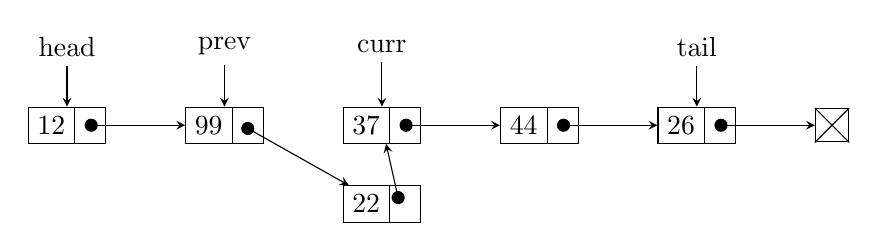
\begin{tikzpicture}[list/.style={rectangle split, rectangle split parts=2, draw, rectangle split horizontal}, >=stealth, start chain]

        \node[list,on chain] (A) {12};
        \node[list,on chain] (B) {99};
        \node[list,on chain] (C) {37};
        \node[list,on chain] (D) {44};
        \node[list,on chain] (E) {26};

        \node[list, below of=C] (New) {22};

        \node[above of=A] (H) {head};
        \node[above of=E] (T) {tail};

        \node[above of=C] (Curr) {curr};
        \node[above of=B] (Prev) {prev};

        \node[on chain,draw,inner sep=6pt] (N) {};
        \draw (N.north east) -- (N.south west);
        \draw (N.north west) -- (N.south east);

        \draw[*->] let \p1 = (A.two), \p2 = (A.center) in (\x1,\y2) -- (B);
        \draw[*->] let \p1 = (B.two), \p2 = (B.center) in (\x1,\y2) -- (New);
        \draw[*->] let \p1 = (New.two), \p2 = (New.center) in (\x1,\y2) -- (C);
        \draw[*->] let \p1 = (C.two), \p2 = (C.center) in (\x1,\y2) -- (D);
        \draw[*->] let \p1 = (D.two), \p2 = (D.center) in (\x1,\y2) -- (E);
        \draw[*->] let \p1 = (E.two), \p2 = (E.center) in (\x1,\y2) -- (N);

        \draw[->] (Curr) -- (C);
        \draw[->] (Prev) -- (B);

        \draw[->] (H) -- (A);
        \draw[->] (T) -- (E);


    \end{tikzpicture}\\
    \textbf{Step 3: Update the new nodes net node to be a reference to the current node}
\end{minipage}




\caption{Add node to the middle of a non-empty LinkedList}
\label{fig:addtomiddle}
\end{figure}

\paragraph{\lstinline|public void addNodeAtPosition(int pos, E data)|}: This
method should instantiate a new node with the data passed in as a parameter
and insert it at a given position. Completing this method has three distinct
stages:\\

\begin{enumerate}
\item In the event \lstinline|pos| is not a valid index (e.g., pos\ > \ size or pos \ < 0) the method should throw an \lstinline|IndexOutOfBoundsException|.

\item If the node position (\lstinline|pos|) is the front (Case 1; pos == 0) or the end (Case 2; pos == size) it should call the appropriate method (i.e., addToFront, addToBack) to insert node.\\

\item If it is somewhere in the middle of the list (e.g., 0 < pos < size) it should search for the node that currently occupies that position and insert the new node before it (Case 3; Figure~\ref{fig:addtomiddle}). As a reminder, this is  where we can use \lstinline|getNodeAtPosition(pos)| and \lstinline|getNodeAtPosition(pos - 1)| to get \lstinline|curr| and \lstinline|prev| respectively.
\end{enumerate}

\subsection*{Testing}
The provided tests for get node at position should output the following after you have implemented this method:
\begin{shell}
addNodeAtPosition Tests
List 3: 1 --> 2 --> 3 --> 2 --> 1 --> null
------------------------------------------
\end{shell}
As was the case with the last one, you should review the test code in
SinglyLinkedListTest.java and add a few more.

\newpage

\section{Step 4: removeFromFront and removeFromEnd}

\begin{figure}[H]
\begin{minipage}{0.48\textwidth}
    \centering
    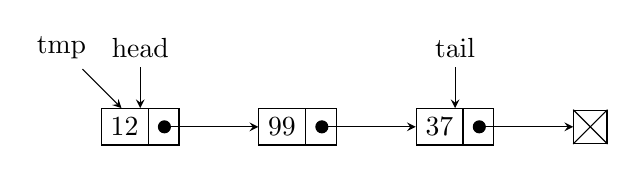
\begin{tikzpicture}[list/.style={rectangle split, rectangle split parts=2, draw, rectangle split horizontal}, >=stealth, start chain]

        \node[list,on chain] (A) {12};
        \node[list,on chain] (B) {99};
        \node[list,on chain] (C) {37};
        \node[above of=A] (H) {head};
        \node[above of=C] (T) {tail};
        \node[left of=H] (Tmp) {tmp};
        \node[on chain,draw,inner sep=6pt] (D) {};
        \draw (D.north east) -- (D.south west);
        \draw (D.north west) -- (D.south east);
        \draw[*->] let \p1 = (A.two), \p2 = (A.center) in (\x1,\y2) -- (B);
        \draw[*->] let \p1 = (B.two), \p2 = (B.center) in (\x1,\y2) -- (C);
        \draw[*->] let \p1 = (C.two), \p2 = (C.center) in (\x1,\y2) -- (D);
        \draw[->] (H) -- (A);
        \draw[->] (T) -- (C);
        \draw[->] (Tmp) -- (A);

    \end{tikzpicture}\\
    \textbf{Step 1: Create a \lstinline|tmp| that references the same node as \lstinline|head|}
\end{minipage}
\hfill
\begin{minipage}{0.48\textwidth}
    \centering
    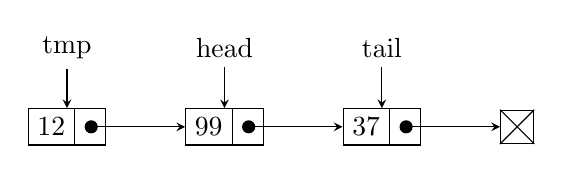
\begin{tikzpicture}[list/.style={rectangle split, rectangle split parts=2, draw, rectangle split horizontal}, >=stealth, start chain]

        \node[list,on chain] (A) {12};
        \node[list,on chain] (B) {99};
        \node[list,on chain] (C) {37};
        \node[above of=B] (H) {head};
        \node[above of=C] (T) {tail};
        \node[above of=A] (Tmp) {tmp};
        \node[on chain,draw,inner sep=6pt] (D) {};
        \draw (D.north east) -- (D.south west);
        \draw (D.north west) -- (D.south east);
        \draw[*->] let \p1 = (A.two), \p2 = (A.center) in (\x1,\y2) -- (B);
        \draw[*->] let \p1 = (B.two), \p2 = (B.center) in (\x1,\y2) -- (C);
        \draw[*->] let \p1 = (C.two), \p2 = (C.center) in (\x1,\y2) -- (D);
        \draw[->] (H) -- (B);
        \draw[->] (T) -- (C);
        \draw[->] (Tmp) -- (A);

    \end{tikzpicture}\\
    \textbf{Step 2: Advance the head pointer}
\end{minipage}\\
\vspace{0.25cm}\\
\begin{minipage}{\textwidth}
    \centering
    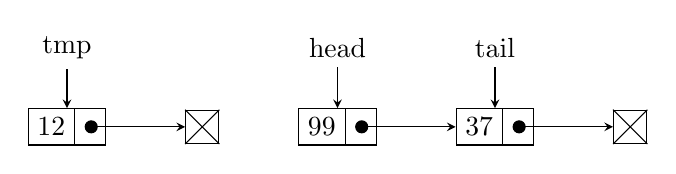
\begin{tikzpicture}[list/.style={rectangle split, rectangle split parts=2, draw, rectangle split horizontal}, >=stealth, start chain]

        \node[list,on chain] (A) {12};

        \node[on chain,draw,inner sep=6pt] (N1) {};
        \draw (N1.north east) -- (N1.south west);
        \draw (N1.north west) -- (N1.south east);

        \node[list,on chain] (B) {99};
        \node[list,on chain] (C) {37};
        \node[above of=B] (H) {head};
        \node[above of=C] (T) {tail};
        \node[above of=A] (Tmp) {tmp};


        \node[on chain,draw,inner sep=6pt] (D) {};
        \draw (D.north east) -- (D.south west);
        \draw (D.north west) -- (D.south east);
        \draw[*->] let \p1 = (A.two), \p2 = (A.center) in (\x1,\y2) -- (N1);
        \draw[*->] let \p1 = (B.two), \p2 = (B.center) in (\x1,\y2) -- (C);
        \draw[*->] let \p1 = (C.two), \p2 = (C.center) in (\x1,\y2) -- (D);
        \draw[->] (H) -- (B);
        \draw[->] (T) -- (C);
        \draw[->] (Tmp) -- (A);

    \end{tikzpicture}\\
    \textbf{Step 3: Remove the reference from the old head to the next head}
\end{minipage}



\caption{Removing a node from the front of a non-empty LinkedList}
\label{fig:removefromfront}
\end{figure}

\paragraph{\lstinline|public void removeFromFront()|: } As the name suggests
you will implement a method that removes the node from the front of the
linked-list. Implementing this method has three cases to consider: 
\begin{enumerate}
 \item If the list is empty, the method should throw \lstinline|IndexOutOfBoundsException|. 
 \item If the list has one item (e.g, \lstinline|head| == \lstinline|tail|) we must set the \lstinline|head| AND \lstinline|tail| to null.
 \item Otherwise, we remove and update the head pointer as shown in Figure~\ref{fig:removefromfront}.
\end{enumerate}

\begin{figure}[H]
\begin{minipage}{0.48\textwidth}
    \centering
    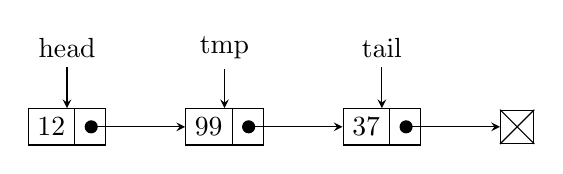
\begin{tikzpicture}[list/.style={rectangle split, rectangle split parts=2, draw, rectangle split horizontal}, >=stealth, start chain]

        \node[list,on chain] (A) {12};

        \node[list,on chain] (B) {99};

        \node[list,on chain] (C) {37};

        \node[above of=A] (H) {head};
        \node[above of=B] (Tmp) {tmp};
        \node[above of=C] (T) {tail};

        \node[on chain,draw,inner sep=6pt] (D) {};
        \draw (D.north east) -- (D.south west);
        \draw (D.north west) -- (D.south east);
        \draw[*->] let \p1 = (A.two), \p2 = (A.center) in (\x1,\y2) -- (B);
        \draw[*->] let \p1 = (B.two), \p2 = (B.center) in (\x1,\y2) -- (C);
        \draw[*->] let \p1 = (C.two), \p2 = (C.center) in (\x1,\y2) -- (D);

        \draw[->] (H) -- (A);
        \draw[->] (Tmp) -- (B);
        \draw[->] (T) -- (C);



    \end{tikzpicture}\\
    \textbf{Step 1: Find the second to last node in the list (i.e., the tail's parent)}
\end{minipage}
\hfill
\begin{minipage}{0.48\textwidth}
    \centering
    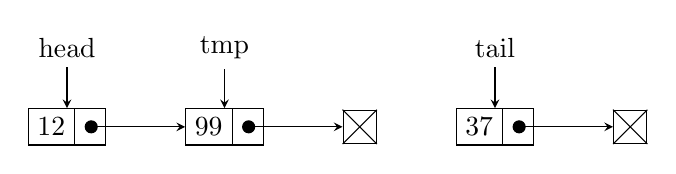
\begin{tikzpicture}[list/.style={rectangle split, rectangle split parts=2, draw, rectangle split horizontal}, >=stealth, start chain]

        \node[list,on chain] (A) {12};

        \node[list,on chain] (B) {99};

        \node[on chain,draw,inner sep=6pt] (N1) {};
        \draw (N1.north east) -- (N1.south west);
        \draw (N1.north west) -- (N1.south east);

        \node[list,on chain] (C) {37};

        \node[above of=A] (H) {head};
        \node[above of=B] (Tmp) {tmp};
        \node[above of=C] (T) {tail};

        \node[on chain,draw,inner sep=6pt] (D) {};
        \draw (D.north east) -- (D.south west);
        \draw (D.north west) -- (D.south east);
        \draw[*->] let \p1 = (A.two), \p2 = (A.center) in (\x1,\y2) -- (B);
        \draw[*->] let \p1 = (B.two), \p2 = (B.center) in (\x1,\y2) -- (N1);
        \draw[*->] let \p1 = (C.two), \p2 = (C.center) in (\x1,\y2) -- (D);

        \draw[->] (H) -- (A);
        \draw[->] (Tmp) -- (B);
        \draw[->] (T) -- (C);

    \end{tikzpicture}\\
    \textbf{Step 2: Detach the tail}
\end{minipage}\\
\vspace{0.25cm}\\
\begin{minipage}{\textwidth}
    \centering
    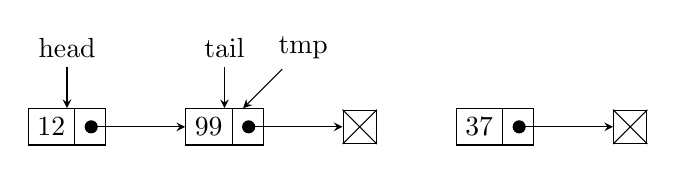
\begin{tikzpicture}[list/.style={rectangle split, rectangle split parts=2, draw, rectangle split horizontal}, >=stealth, start chain]

        \node[list,on chain] (A) {12};

        \node[list,on chain] (B) {99};

        \node[on chain,draw,inner sep=6pt] (N1) {};
        \draw (N1.north east) -- (N1.south west);
        \draw (N1.north west) -- (N1.south east);

        \node[list,on chain] (C) {37};

        \node[above of=A] (H) {head};
        \node[above of=B] (T) {tail};
        \node[right of=T] (Tmp) {tmp};

        \node[on chain,draw,inner sep=6pt] (D) {};
        \draw (D.north east) -- (D.south west);
        \draw (D.north west) -- (D.south east);
        \draw[*->] let \p1 = (A.two), \p2 = (A.center) in (\x1,\y2) -- (B);
        \draw[*->] let \p1 = (B.two), \p2 = (B.center) in (\x1,\y2) -- (N1);
        \draw[*->] let \p1 = (C.two), \p2 = (C.center) in (\x1,\y2) -- (D);

        \draw[->] (H) -- (A);
        \draw[->] (T) -- (B);
        \draw[->] (Tmp) -- (B);
    \end{tikzpicture}\\
    \textbf{Step 3: Update the tail reference}
\end{minipage}



\caption{Removing a node to the end of a non-empty LinkedList}
\label{fig:removefromback}
\end{figure}

\paragraph{\lstinline|public void removeFromEnd(E data)|: } Similar to
\lstinline|removeFromFront| you will implement a method that removes the node from the
back of the linked-list. This also has three cases to consider:
\begin{enumerate}
 \item Again, if the list is empty, the method should throw \lstinline|IndexOutOfBoundsException|. 
 \item If the list has one item (e.g, \lstinline|head| == \lstinline|tail|) we must set the \lstinline|head| AND \lstinline|tail| to null.
 \item Otherwise, we remove and update the head pointer (see Figure~\ref{fig:removefromfront}). For this, you can once again your \lstinline|getNodeAtPosition| method you implemented earlier to get the second to last node.
\end{enumerate}

\subsection*{Testing}
The provided tests for get node at position should output the following after you have implemented this method:
\begin{shell}
Remove from front of List 1
List 1 after front removal: 2 --> 1 --> null

Remove from end of List 2
List 2 after front removal: 1 --> 2 --> null
\end{shell}

\newpage

\section{Step 5: removeNodeAtPostion}

\begin{figure}[H]
\begin{minipage}{\textwidth}
    \centering
    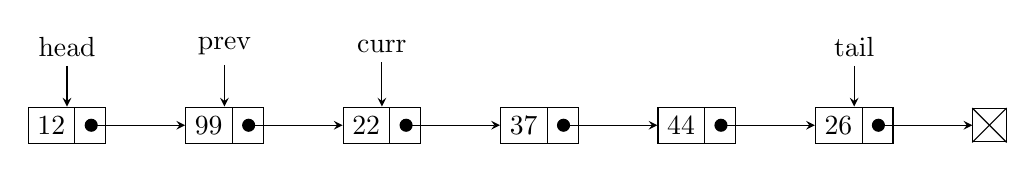
\begin{tikzpicture}[list/.style={rectangle split, rectangle split parts=2, draw, rectangle split horizontal}, >=stealth, start chain]

        \node[list,on chain] (A) {12};
        \node[list,on chain] (B) {99};
        \node[list,on chain] (C) {22};
        \node[list,on chain] (D) {37};
        \node[list,on chain] (E) {44};
        \node[list,on chain] (F) {26};


        \node[above of=A] (H) {head};
        \node[above of=F] (T) {tail};

        \node[above of=C] (Curr) {curr};
        \node[above of=B] (Prev) {prev};

        \node[on chain,draw,inner sep=6pt] (N) {};
        \draw (N.north east) -- (N.south west);
        \draw (N.north west) -- (N.south east);

        \draw[*->] let \p1 = (A.two), \p2 = (A.center) in (\x1,\y2) -- (B);
        \draw[*->] let \p1 = (B.two), \p2 = (B.center) in (\x1,\y2) -- (C);
        \draw[*->] let \p1 = (C.two), \p2 = (C.center) in (\x1,\y2) -- (D);
        \draw[*->] let \p1 = (D.two), \p2 = (D.center) in (\x1,\y2) -- (E);
        \draw[*->] let \p1 = (E.two), \p2 = (E.center) in (\x1,\y2) -- (F);
        \draw[*->] let \p1 = (F.two), \p2 = (F.center) in (\x1,\y2) -- (N);

        \draw[->] (Curr) -- (C);
        \draw[->] (Prev) -- (B);

        \draw[->] (H) -- (A);
        \draw[->] (T) -- (F);

    \end{tikzpicture}\\
    \textbf{Step 1: Search for and find a reference to the node you want to remove and the node that precedes it.}
\end{minipage}
\begin{minipage}{\textwidth}
    \centering
    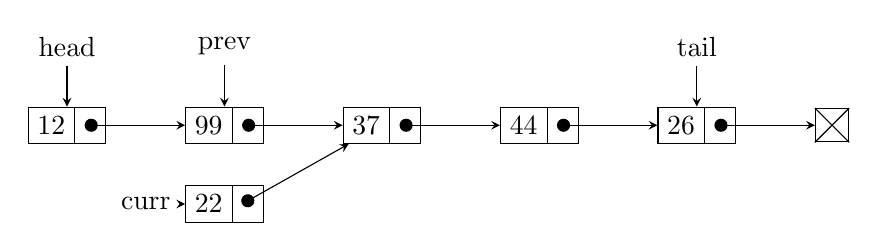
\begin{tikzpicture}[list/.style={rectangle split, rectangle split parts=2, draw, rectangle split horizontal}, >=stealth, start chain]

        \node[list,on chain] (A) {12};
        \node[list,on chain] (B) {99};
        \node[list, below of=B] (C) {22};
        \node[list,on chain] (D) {37};
        \node[list,on chain] (E) {44};
        \node[list,on chain] (F) {26};


        \node[above of=A] (H) {head};
        \node[above of=F] (T) {tail};

        \node[left of=C] (Curr) {curr};
        \node[above of=B] (Prev) {prev};

        \node[on chain,draw,inner sep=6pt] (N) {};
        \draw (N.north east) -- (N.south west);
        \draw (N.north west) -- (N.south east);

        \draw[*->] let \p1 = (A.two), \p2 = (A.center) in (\x1,\y2) -- (B);
        \draw[*->] let \p1 = (B.two), \p2 = (B.center) in (\x1,\y2) -- (D);
        \draw[*->] let \p1 = (C.two), \p2 = (C.center) in (\x1,\y2) -- (D);
        \draw[*->] let \p1 = (D.two), \p2 = (D.center) in (\x1,\y2) -- (E);
        \draw[*->] let \p1 = (E.two), \p2 = (E.center) in (\x1,\y2) -- (F);
        \draw[*->] let \p1 = (F.two), \p2 = (F.center) in (\x1,\y2) -- (N);

        \draw[->] (Curr) -- (C);
        \draw[->] (Prev) -- (B);

        \draw[->] (H) -- (A);
        \draw[->] (T) -- (F);

    \end{tikzpicture}\\
    \textbf{Step 2: Update previous node's next node to be the current nodes next node.}
\end{minipage}\\
\vspace{0.25cm}\\
\begin{minipage}{\textwidth}
    \centering
    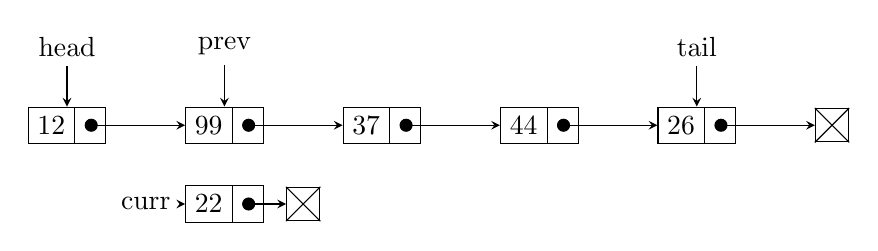
\begin{tikzpicture}[list/.style={rectangle split, rectangle split parts=2, draw, rectangle split horizontal}, >=stealth, start chain]

        \node[list,on chain] (A) {12};
        \node[list,on chain] (B) {99};
        \node[list, below of=B] (C) {22};
        \node[list,on chain] (D) {37};
        \node[list,on chain] (E) {44};
        \node[list,on chain] (F) {26};


        \node[above of=A] (H) {head};
        \node[above of=F] (T) {tail};

        \node[left of=C] (Curr) {curr};
        \node[above of=B] (Prev) {prev};

        \node[on chain,draw,inner sep=6pt] (N) {};
        \draw (N.north east) -- (N.south west);
        \draw (N.north west) -- (N.south east);


        \node[right of=C, draw,inner sep=6pt] (N1) {};
        \draw (N1.north east) -- (N1.south west);
        \draw (N1.north west) -- (N1.south east);

        \draw[*->] let \p1 = (A.two), \p2 = (A.center) in (\x1,\y2) -- (B);
        \draw[*->] let \p1 = (B.two), \p2 = (B.center) in (\x1,\y2) -- (D);
        \draw[*->] let \p1 = (C.two), \p2 = (C.center) in (\x1,\y2) -- (N1);
        \draw[*->] let \p1 = (D.two), \p2 = (D.center) in (\x1,\y2) -- (E);
        \draw[*->] let \p1 = (E.two), \p2 = (E.center) in (\x1,\y2) -- (F);
        \draw[*->] let \p1 = (F.two), \p2 = (F.center) in (\x1,\y2) -- (N);

        \draw[->] (Curr) -- (C);
        \draw[->] (Prev) -- (B);

        \draw[->] (H) -- (A);
        \draw[->] (T) -- (F);


    \end{tikzpicture}\\
    \textbf{Step 3: Null out the current nodes next node to fully remove it from the list}
\end{minipage}

\caption{Removing a node from the middle of a non-empty LinkedList}
\label{fig:removefrommiddle}
\end{figure}

\paragraph{\lstinline|public void removeNodeAtPosition(int pos)|}: This
method should find the node at a given position. If the node position is at
the head (Case 1; pos == 0) or at the end (Case 2; pos == size - 1) it should
call the appropriate method to remove that node (i.e., the ones you implemented
at the beginning of the assessment). If it is somewhere in the middle of the
list (e.g., 0 < pos < size -1) it should search for that node and remove it
(Case 3; Figure~\ref{fig:addtomiddle}). In the event pos is not a valid index
(e.g., pos\ > \ size - 1 or pos is negative) the method should throw an
\lstinline|IndexOutOfBoundsException|.\\

\begin{shell}
Remove position (front, end, middle) from List 3
List 3 after removing middle, front, and end: 2 --> 2 --> null
\end{shell}

\newpage

%\textbf{toString Override}\\
%
%Here, it will once again be useful to have a toString overide so we can easily print 
%our lists. Construct the method such that it iterates over each list node, retrieves
%the data, and returns a string with each values separated by a \lstinline|->|. As 
%and example:
%
%\begin{framed}
%\begin{minipage}{0.6\textwidth}
%\underline{\textbf{Main.java}}
%\begin{lstlisting}
%public class Main{
%    SinglyLinkedList<Integer> list = new SinglyLinkedList<Integer>();
%    //Add 1, 2, 3
%    System.out.println(list);
%}
%\end{lstlisting}
%\end{minipage}
%\hfill
%\vline
%\hfill
%\begin{minipage}{0.35\textwidth}
%\underline{\textbf{Terminal:}}
%\begin{shell}
%1 -> 2 -> 3
%\end{shell}
%\end{minipage}
%\end{framed}
%\vspace{0.2cm}
%
%This method will be of particular use to you while you are testing your program.


\newpage
\section{Hints}

For this assignment you will be creating and throwing exceptions when invalid 
operations are attempted to be performed. Exceptions, in Java are created via
two elements:
\begin{enumerate}
	\item The method header specifies that it throws an exception, as shown in the following template: \lstinline|public void foo() throws Exception{ /* ... */}|.
	\item A new exception is created and thrown: \lstinline|throw new Exception()|;
\end{enumerate}
In this assignment you are told at a number of points to throw an  IndexOutOfBoundsException. You are given the 
method headers so all you need to do is use a conditional to determine when the exception should be thrown then
fill in the code that throws the IndexOutOfBoundsException in the body of that if statement. Example code for 
this is shown below.

\begin{lstlisting}[frame=trBL]
public ListNode<E> getNodeAtPosition(int pos) throws IndexOutOfBoundsException{
	if(pos > size - 1 || pos < 0) {
		throw new IndexOutOfBoundsException();
	}
	
	return new ListNode<>((E) new Object()); // Remove this line once you begin to implement this method
}
\end{lstlisting}

\subsection{Checklist}
\begin{itemize}
    \item ListNode: All the stuff here is given to you so check off if you didn't modify it :) 
    \item SinglyLinkedList 
        \begin{todolist}
            \item The following accessors and list modification methods have been implemented:
            \begin{todolist}
                \item \lstinline|getNodeAtPosition|
                \item \lstinline|addToFront|
                \item \lstinline|removeFromFront|
                \item \lstinline|addToEnd|
                \item \lstinline|removeFromEnd|
                \item \lstinline|addNodeAtPosition|
                \item \lstinline|removeNodeAtPosition|
            \end{todolist}
        \end{todolist}
\end{itemize}

%%\newpage
%%\bibliographystyle{apacite}
%%\bibliography{sample}

\end{document}
